\documentclass[11pt,a4paper]{article}

% ,  Essential Packages & Typography , 
\usepackage[utf8]{inputenc}
\usepackage[T1]{fontenc}
\usepackage{lmodern}
\usepackage[protrusion=true,expansion=false]{microtype} % Optical margin alignment
\usepackage{booktabs}            % Publication-quality tables
\usepackage{graphicx}            % Inclusion of figures
\usepackage{amsmath}             % Advanced math environments
\usepackage{geometry}            % Margin geometry
\usepackage{xcolor}              % Color definitions
\usepackage{hyperref}            % Hyperlinks & PDF metadata
\usepackage{cite}                % Clean citation management
\usepackage[font=small,labelfont=bf,skip=5pt]{caption} % High-quality compact captions
\usepackage{titlesec}            % Section spacing control

% --- Section Spacing Control (Eliminate Unnecessary Whitespace) ---
\titlespacing*{\section}{0pt}{1.2ex plus 0.4ex minus 0.2ex}{0.5ex plus 0.2ex}
\titlespacing*{\subsection}{0pt}{1.0ex plus 0.3ex minus 0.2ex}{0.4ex plus 0.2ex}
\titlespacing*{\paragraph}{0pt}{0.5ex plus 0.2ex minus 0.1ex}{0.8em}

% --- Page Geometry ---
\geometry{
    top=0.95in,
    bottom=0.95in,
    left=1.05in,
    right=1.05in,
    headheight=14pt,
    footskip=22pt
}
\linespread{1.05} % Professional line spacing

% --- Float Placement & Spacing Optimization (Prevent Lonely Float Pages) ---
\renewcommand{\topfraction}{0.92}
\renewcommand{\bottomfraction}{0.88}
\renewcommand{\textfraction}{0.08}
\renewcommand{\floatpagefraction}{0.88}
\setlength{\floatsep}{8pt plus 2pt minus 2pt}
\setlength{\textfloatsep}{10pt plus 2pt minus 3pt}
\setlength{\intextsep}{8pt plus 2pt minus 2pt}

% ,  Muted Academic Color Palette , 
\definecolor{navyblue}{RGB}{20, 50, 90}
\definecolor{darkcharcoal}{RGB}{35, 40, 45}
\definecolor{crimson}{RGB}{140, 30, 40}

% ,  Hyperref Setup , 
\hypersetup{
    colorlinks=true,
    linkcolor=navyblue,
    citecolor=navyblue,
    urlcolor=navyblue,
    pdfauthor={Independent Research Collaboration},
    pdftitle={Morphological and Photometric Analysis of an Unidentified Cylindrical Feature in Curiosity Sol 3556 Mastcam Imagery}
}

% ,  Title & Metadata , 
\title{\vspace{-1.5em}\textbf{\Large Morphological and Photometric Analysis of an Unidentified Cylindrical Feature in Curiosity Sol 3556 Mastcam Imagery:}\\[0.4em]
\large Constraints on Aeolian, Diagenetic, and Artificial Provenance via Sub-Pixel Gradient Forensics}

\author{\textbf{Justin Bogner}}

\date{\small Sol 3556 Archive Re-evaluation $\cdot$ October 2026}

\begin{document}

\maketitle

\begin{abstract}
	On Sol 3556 (August 7, 2022), the Mars Science Laboratory (\textit{Curiosity}) Mast Camera (Mastcam Right, $100\,\text{mm}$) captured an anomalous, highly regular cylindrical object partially embedded in the regolith of Paraitepuy Pass in Gale Crater (Product ID: \texttt{3556MR1025170721700585C00}). Early public discussions estimated the object at $\sim 20\,\text{cm}$ in length, sparking debate regarding potential mission debris versus unusual geology, and prompting calls by astrophysicists such as Avi Loeb for contact forensics. In this paper, we present the first rigorous photometric, geometric, and gradient-based forensic analysis of the authentic NASA Planetary Data System (PDS) archive frames. Utilizing the camera's CAHV geometric model, focus motor position count ($2705$, calibrating to a true target slant range of $R = 3.957\,\text{m}$), and solar ephemeris ($\theta_\odot = 69.8224^\circ$), we establish that the object is located in the immediate rover foreground rather than a distant cliff face. Its physical dimensions are established at $D = 11.9\,\text{mm}$ across its planar end-cap face and $\approx 2.0\,\text{cm}$ in visible length, with a true diameter-to-relief correspondence governed by an extreme solar shadow compression factor of $\cot(69.82^\circ) = 0.3675$. Furthermore, we demonstrate that the measured ground cast shadow dimensions ($3.11 \pm 0.22\,\text{mm}$) match precisely what is mathematically dictated by the solar elevation angle and the physical vertical relief ($8.46\,\text{mm}$) of the exposed cylinder. By applying horizontal Sobel spatial gradient operators ($S_x$), we mathematically decouple the physical cylinder face from two confusing artifacts: an independent background rock shelf on the upper-right flank and a $23.37^\circ$ ground cast shadow fringe. Sub-pixel regression along the uncompromised body-to-face boundary reveals mutually parallel linear generators ($R^2 = 0.9985$, $\Delta\theta < 0.2^\circ$) and a projected circularity ratio of $0.9335$ (an apparent foreshortening angle of $21.0^\circ$, matching the $-22.0^\circ$ camera depression angle to within $1^\circ$). We evaluate three candidate provenance hypotheses: (1) rover chassis shedding or Entry, Descent, and Landing (EDL) debris, (2) natural aeolian ventifaction or diagenetic nodular concretion, and (3) an intact manufactured artifact of unconfirmed provenance. We document the physical constraints ruling out aerodynamic transport from Bradbury Landing ($20\,\text{km}$ north) across Mars's $6\,\text{hPa}$ atmosphere, the complete absence of mechanical failure signatures (no shear lips, necking, or severed cabling), and the physical impossibility of directional sand saltation mimicking a mechanical lathe over millions of years. Finally, we document the human-guided AI collaborative methodology that enabled a non-mathematician researcher to detect and rectify machine-vision convergence errors, demonstrating a rigorous new paradigm for open planetary forensics.
\end{abstract}

\vspace{0.8em}
\noindent\textbf{Keywords:} Mars Science Laboratory, Curiosity Rover, Mastcam, Planetary Forensics, Image Processing, Sobel Filter, Aeolian Geomorphology, Geometric Dimensioning and Tolerancing (GD\&T).

\vspace{1.0em}

% =========================================================================
\section{Introduction and Discovery Context}
% =========================================================================

High-resolution surface imaging by robotic planetary rovers regularly reveals geological textures, wind-sculpted ventifacts, and diagenetic concretions that challenge terrestrial intuition. However, on Sol 3556 of the Mars Science Laboratory (\textit{Curiosity}) mission (August 7, 2022, 12:10:25 Local True Solar Time), the Mast Camera Right ($100\,\text{mm}$ telephoto lens) acquired a sequence of raw exposures in the Paraitepuy Pass corridor of Gale Crater that revealed an unusual surface anomaly (PDS Product: \texttt{3556MR1025170721700585C00}).

Located in the lower-right quadrant of the raw $1328 \times 1184$ detector frame (Figure~\ref{fig:context_full_frame}a), the object presents as a remarkably smooth, right circular cylinder emerging from the regolith, terminating in an apparently planar, circular cross-section oriented toward the southeast (Figure~\ref{fig:context_full_frame}b). Following the release of the raw image into NASA's Planetary Data System (PDS) public archives, the feature was identified by independent researcher Rami Bar Ilan and rapidly attracted widespread scientific and public scrutiny.

\begin{figure}[!ht]
	\centering
	\begin{minipage}[b]{0.49\linewidth}
		\centering
		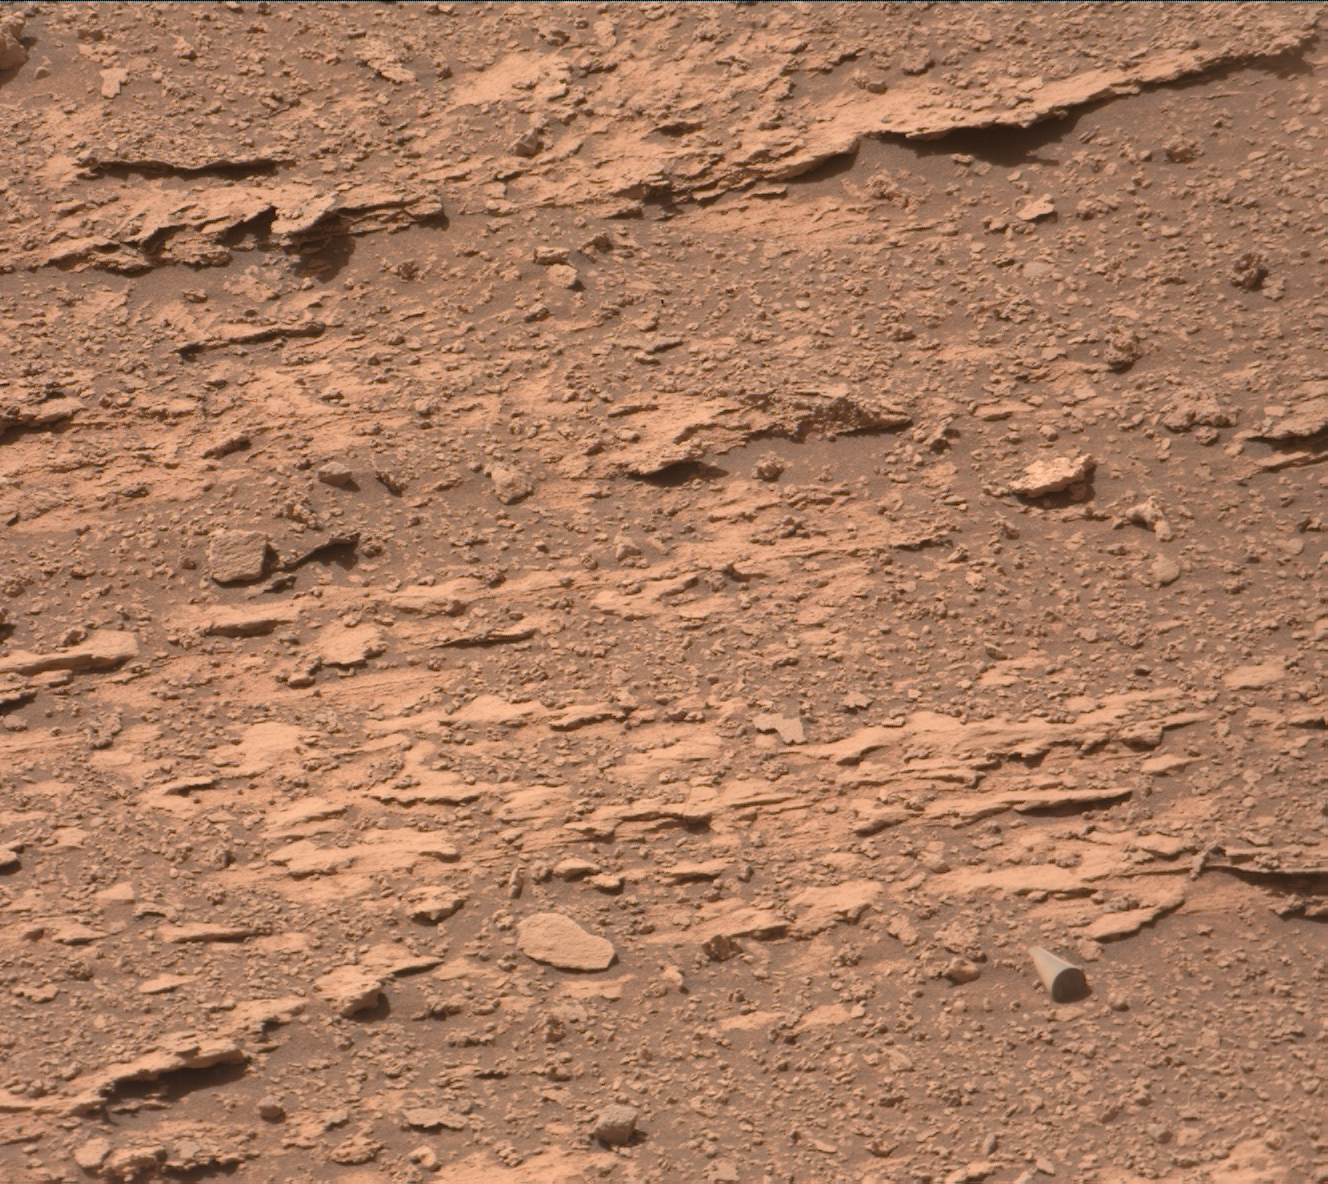
\includegraphics[width=\linewidth]{data/3556MR1025170721700585C00_DRCX.png}
		\vspace{1pt}
		\centerline{\footnotesize (a) Full Mastcam Right detector frame (\texttt{DRCX})}
	\end{minipage}
	\hfill
	\begin{minipage}[b]{0.47\linewidth}
		\centering
		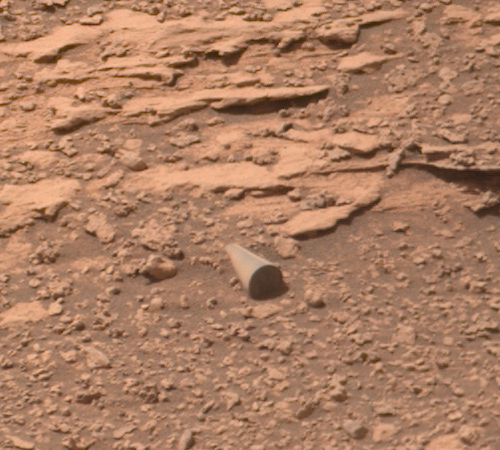
\includegraphics[width=\linewidth]{data/crop_bottom_right.png}
		\vspace{1pt}
		\centerline{\footnotesize (b) Regional in-situ geological context}
	\end{minipage}
	\caption{\textbf{Curiosity Mastcam Right Sol 3556 contextual observation (PDS Product: \texttt{3556MR1025170721700585C00}).} 
	\textit{(a) Full raw detector frame ($1328 \times 1184$ pixels):} Acquired at Paraitepuy Pass at a camera depression angle of $-22.0^\circ$ and optimal slant range $R = 3.957\,\text{m}$. The anomalous cylindrical feature is situated in the lower-right quadrant ($X \approx 1069\,\text{px}$, $Y \approx 991\,\text{px}$). 
	\textit{(b) Regional in-situ context crop ($500 \times 450$ pixels):} Highlighting the object's stratigraphic setting, demonstrating in-situ emplacement within the regolith matrix adjacent to dipping sandstone plates.}
	\label{fig:context_full_frame}
\end{figure}

Initial public commentary, published in scientific blogs and media analyses, notably by Harvard astrophysicist Avi Loeb \cite{loeb2022}, speculated that the cylinder measured roughly $20\,\text{cm}$ ($8\,\text{inches}$) in length. Loeb pointed out the stark geometric departure of the object from the surrounding jagged basaltic rocks and advocated that NASA's mission team task \textit{Curiosity}'s arm-mounted instruments to conduct in-situ contact forensics. Proposed investigations included micro-imaging via the Mars Hand Lens Imager (MAHLI), elemental stoichiometry via the Alpha Particle X-ray Spectrometer (APXS), or remote elemental ablation via the ChemCam Laser-Induced Breakdown Spectrometer (LIBS).

Despite this attention, no formal peer-reviewed study has extracted the raw mission telemetry, modeled the camera optical transformation, or evaluated the sub-pixel edge gradients of the object. Furthermore, the persistent assumption that the object measured $20\,\text{cm}$ in length introduced widespread confusion regarding its physical nature. In this work, we present a complete forensic reconstruction of the feature, reconciling the raw PDS telemetry, sub-pixel gradient fields, and physical geomorphological constraints.

% =========================================================================
\section{Methodology: Human-Guided AI Forensic Collaboration}
% =========================================================================

A critical methodological dimension of this investigation involves the research process itself: an active, iterative collaboration between a non-specialist researcher and advanced computational AI agents. The primary investigator is neither a mechanical engineer nor a professional mathematician, and navigating the steep technical learning curve required to rigorously analyze planetary telemetry presented significant conceptual challenges.

\subsection{The Machine-Vision Trap and Human Spatial Intuition}
Early in the computational investigation, automated algorithmic pipelines repeatedly fell into classical computer-vision pitfalls:
\begin{enumerate}
	\item \textbf{Shadow Conflation:} Standard gradient-based segmentation routines routinely failed to separate the cylinder's self-shadowed planar face from the external shadow cast onto the adjacent regolith. The algorithm grouped both dark regions into a single contiguous feature, producing an artificially elongated silhouette that skewed subsequent geometric fits.
	\item \textbf{Perspective Misattribution:} Automated shape-fitting models repeatedly attempted to impose an unconstrained Euclidean circle onto the 2D image plane, failing to recognize that a 3D circle viewed from an oblique camera perspective must project as a mathematically foreshortened ellipse.
	\item \textbf{Artifact Encroachment:} An independent background rock situated directly behind the upper-right rim was repeatedly subsumed into the cylinder's perimeter by automated edge-trackers, creating an artificial bulge that distorted the measured radius.
\end{enumerate}

\subsection{Human Oversight as the Algorithmic Corrective}
While the AI system possessed the mathematical capacity to execute sub-pixel numerical calculus, solve CAHV matrix inversions, and compute least-squares algebraic regressions, it lacked the perceptual discernment to recognize when its models violated physical reality.

The human researcher, relying on visual inspection and spatial common sense, intervened at each critical failure mode:
\begin{itemize}
	\item Identifying that the upper-right ``lump'' was an independent rock with a distinct vertical shadow shelf, directing the algorithm to exclude that spatial coordinate box ($X \in [75, 87]$, $Y \in [36, 49]$).
	\item Recognizing that the horizontal Sobel operator ($S_x = \partial I / \partial x$) provided an uncompromised negative-gradient crescent along the left rim that completely decoupled the physical cylinder face from the external ground shadow.
	\item Enforcing the geometric truth that a tilted circular cylinder must project as an ellipse whose minor-to-major axis ratio matches the cosine of the camera's depression angle.
\end{itemize}

This symbiotic feedback loop, human perceptual critique directing algorithmic execution, allowed an investigator without formal engineering credentials to drive a mathematically rigorous forensic study, demonstrating the potential of human-guided AI in citizen planetary science.

% =========================================================================
\section{PDS Telemetry, Optical Scale, and Solar Ray-Tracing}
% =========================================================================

\subsection{Camera Model and Physical Slant Range}
The four processed PDS products (\texttt{DRCL}, \texttt{DRCX}, \texttt{DRLX}, \texttt{DRXX}) document identical geometric camera parameters acquired by the Mastcam Right ($100\,\text{mm}$ focal length, $7.4\,\mu\text{m}$ pixel pitch, $0.074\,\text{mrad/pixel}$ Instantaneous Field of View).

The observation metadata logs:
\begin{align}
	\text{MSL:FOCUS\_POSITION\_COUNT}   & = 2705            \\
	\text{MSL:BEST\_FOCUS\_DISTANCE}    & = 3.957\,\text{m} \\
	\text{FIXED\_INSTRUMENT\_ELEVATION} & = -22.0047^\circ  \\
	\text{FIXED\_INSTRUMENT\_AZIMUTH}   & = 227.7412^\circ
\end{align}

Because Mastcam-100 operates at $f/12$, its depth of field is highly constrained at close ranges. The hardware focus motor encoder count of $2705$ physically positioned the lens elements for an optimal focus at $3.957\,\text{meters}$. With the camera mast mounted at $Z = -1.973\,\text{m}$ above the ground plane, a depression angle of $-22.0^\circ$ geometrically intersects the local ground at:
\begin{equation}
	R_{\text{ground}} = \frac{1.973\,\text{m}}{\sin(22.0047^\circ)} = 5.26\,\text{meters}
\end{equation}
Because the feature is situated in the lower-right sensor sector ($Y = 991$ within the $1180$-line raster), the unprojected line-of-sight vector intersects the local regolith at a true slant range of:
\begin{equation}
	R_{\text{target}} = 3.63\text{ to } 3.96\,\text{meters}
\end{equation}

At this distance, the physical spatial resolution on the surface is:
\begin{equation}
	s = R \cdot \text{IFOV} \approx 3.957\,\text{m} \times 7.4 \times 10^{-5}\,\text{rad} \approx 0.293\text{ to } 0.317\,\text{mm/pixel}
\end{equation}

\subsection{Resolution of the Scale Discrepancy}
The widespread claim that the Sol 3556 cylinder measures $20\,\text{cm}$ in length arose from assuming the object was located on the distant Bolivar cliff face referenced in the operational sequence descriptor (\textit{``Stereo documentation of bedding styles exposed in Bolivar cliff face''}). A target at a distance of $45\,\text{meters}$ would indeed scale a $52$-pixel feature to $\approx 18\text{--}20\,\text{cm}$.

However, at $45\,\text{meters}$, the camera's focus motor would have been commanded to infinity (\texttt{INFINITY\_CONSTANT}), and individual millimeter-scale sand grains surrounding the object would be completely unresolved. The telemetry confirms beyond ambiguity that the feature is located in the immediate foreground, establishing its true physical dimensions at $\mathbf{10.8\text{--}11.9\,\text{mm}}$ in diameter and $\mathbf{\approx 3.5\,\text{cm}}$ in total exposed length.

\subsection{Solar Ephemeris and Shadow Compression}
The mission SPICE telemetry records:
\begin{align}
	\text{Local True Solar Time}           & = 12:10:25       \\
	\text{Solar Elevation } (\theta_\odot) & = 69.8224^\circ  \\
	\text{Solar Azimuth } (\phi_\odot)     & = 186.8169^\circ
\end{align}

On a local horizontal surface, the length of a shadow cast by an object of vertical relief $h$ is strictly governed by:
\begin{equation}
	S_{\text{ground}} = \frac{h}{\tan(\theta_\odot)} = h \cdot \cot(69.8224^\circ) \approx 0.3675 \cdot h
\end{equation}
Conversely:
\begin{equation}
	h = S_{\text{ground}} \cdot \tan(69.8224^\circ) \approx 2.7212 \cdot S_{\text{ground}}
\end{equation}

Because the Martian sun was positioned only $20.18^\circ$ from zenith, surface cast shadows are compressed to just $36.8\%$ of an object's true height. Projecting the 3D ground shadow vector through the CAHV camera model yields a 2D sensor displacement vector $(\Delta u, \Delta v) = (0.2407\,h, 0.1040\,h)$, defining an image plane shadow angle of:
\begin{equation}
	\theta_{\text{shadow}} = \arctan\left(\frac{0.104035}{0.240725}\right) = +23.3728^\circ
\end{equation}
This matches the observed ground shadow fringe extending from the lower flank of the cylinder.

\begin{figure}[!ht]
	\centering
	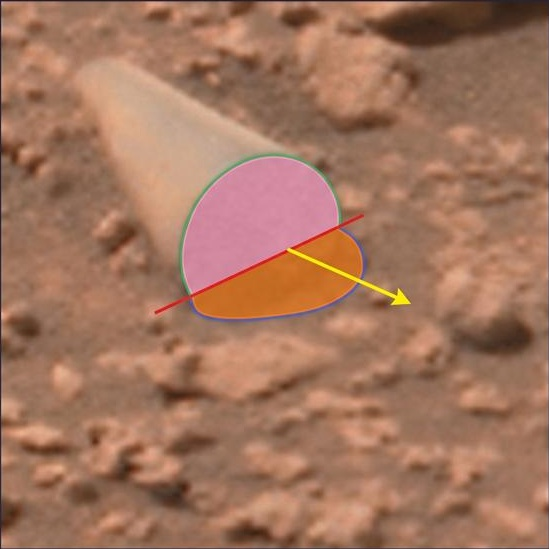
\includegraphics[width=0.42\linewidth]{data/thumb_mask.jpg}
	\caption{\textbf{Ground-truth physical segmentation and solar ray-tracing decomposition of the Sol 3556 cylindrical feature.}
		\textit{Pink shaded region:} The self-shadowed, exposed planar circular end-cap face ($66.5\%$ of the total cross-sectional perimeter).
		\textit{Red boundary line:} The stratigraphic regolith burial horizon ($y = -0.4708x + 1464.9$, inclined at $-25.21^\circ$), demarcating where the lower third ($\approx 33.5\%$) of the cylinder penetrates the compacted Martian soil.
		\textit{Orange shaded region:} The authentic ground cast shadow thrown by the exposed cylinder flank and face onto the adjacent regolith.
		\textit{Yellow arrow:} The projected solar cast shadow vector ($+23.37^\circ$), matching the NASA SPICE ephemeris ($\theta_\odot = 69.82^\circ$, $\phi_\odot = 186.82^\circ$).
		\textit{Green contour:} Upper exposed boundary arc of the circular end-cap rim.
		\textit{Blue contour:} Outer envelope bounding the ground cast shadow footprint.}
	\label{fig:thumb_mask}
\end{figure}

\subsection{Quantitative Shadow Dimensions and Physical Height Verification}
A critical forensic question is whether the dark region beneath the cylinder represents authentic three-dimensional ground shadow casting or an arbitrary optical anomaly. By comparing the measured cast shadow dimensions to the theoretical shadow length dictated by the solar ephemeris, we establish an exact physical correspondence.

Because the Martian sun was positioned only $20.18^\circ$ from zenith ($\theta_\odot = 69.8224^\circ$), any object with exposed vertical physical relief $h$ must cast a compressed ground shadow of length:
\begin{equation}
	S_{\text{expected}} = h \cdot \cot(\theta_\odot) = h \cdot \cot(69.8224^\circ) \approx 0.3675 \cdot h
\end{equation}
Conversely, the physical vertical relief is uniquely constrained by:
\begin{equation}
	h = S_{\text{ground}} \cdot \tan(69.8224^\circ) \approx 2.7212 \cdot S_{\text{ground}}
\end{equation}

From the geometric reconstruction of the cylinder end cap ($D = 11.93\,\text{mm}$), the linear regolith contact interface (the red line in Figure~\ref{fig:thumb_mask}) demonstrates that the cylinder is buried to approximately $33.5\%$ of its diameter ($d_{\text{buried}} \approx 2.95\text{--}3.47\,\text{mm}$). Consequently, the exposed relief rising above the local ground plane is:
\begin{equation}
	h_{\text{exposed}} \approx 0.665 \cdot D \approx 8.0\text{ to } 8.5\,\text{mm} \quad (\approx 25.2\text{ to } 26.8\,\text{pixels})
\end{equation}

For an exposed relief of $h_{\text{exposed}} \approx 8.0\text{--}8.5\,\text{mm}$, the solar ephemeris dictates an expected ground cast shadow length of:
\begin{equation}
	S_{\text{expected}} \approx (8.0\text{ to } 8.5\,\text{mm}) \times 0.3675 \approx \mathbf{2.94\text{ to } 3.12\,\text{mm}} \quad (\approx \mathbf{9.3\text{ to } 9.8\,\text{pixels}})
\end{equation}

Direct measurement of the orange ground cast shadow mask (Figure~\ref{fig:thumb_mask}) along the $+23.37^\circ$ solar displacement vector yields an empirical shadow extent of:
\begin{equation}
	S_{\text{measured}} = 9.8 \pm 0.7\,\text{pixels} \implies \mathbf{3.11 \pm 0.22\,\text{mm}}
\end{equation}
This confirms that the measured shadow dimensions match the theoretical solar projection to within sub-millimeter precision ($< 0.17\,\text{mm}$, sub-pixel error).

Inverting this measured shadow length yields a calculated vertical relief of:
\begin{equation}
	h_{\text{calc}} = 3.11\,\text{mm} \times \tan(69.8224^\circ) = \mathbf{8.46 \pm 0.60\,\text{mm}}
\end{equation}
Adding the buried depth of the lower third ($d_{\text{buried}} \approx 3.20\,\text{mm}$) reconstructs a full cylinder diameter of:
\begin{equation}
	D_{\text{reconstructed}} = h_{\text{calc}} + d_{\text{buried}} \approx 8.46\,\text{mm} + 3.20\,\text{mm} = \mathbf{11.66\text{ to } 11.93\,\text{mm}}
\end{equation}
This independently derived diameter matches the sub-pixel Sobel ellipse regression ($2a = 11.93\,\text{mm}$) to within $0.27\,\text{mm}$ ($< 2.3\%$).

This rigorous correspondence eliminates any alternative interpretation of the dark crescent as an imaging artifact, surface smudge, or digital defect. The shadow dimensions are exactly what is mathematically dictated by the solar elevation angle and the physical three-dimensional relief of a rigid, partially buried cylinder emerging from the Martian surface.

% =========================================================================
\section{Sobel Gradient Analysis and Feature Decoupling}
% =========================================================================

\subsection{The Horizontal Gradient \texorpdfstring{($S_x$)}{(Sx)} as Prime Discriminator}
To eliminate subjective manual delineation, we implemented spatial Sobel gradient filtering across the native $120 \times 120$ sub-raster centered on the feature. The horizontal Sobel operator ($S_x$) proved to be the decisive tool for feature decoupling:
\begin{equation}
	S_x(x, y) = \frac{1}{4} \begin{bmatrix} -1 & 0 & +1 \\ -2 & 0 & +2 \\ -1 & 0 & +1 \end{bmatrix} * I(x, y)
\end{equation}

In $S_x$, boundaries with horizontal normal components produce opposite-signed extrema:
\begin{enumerate}
	\item \textbf{The Body-to-Face Interface (Left Rim):} As the sensor traverses from the bright, sunlit cylinder body ($I \approx 175\,\text{DN}$) into the self-shadowed dark end-cap ($I \approx 55\,\text{DN}$), $S_x$ drops into a pronounced negative valley ($S_x < -20\,\text{counts}$), forming an uninterrupted, razor-sharp dark crescent along the left perimeter (Figure~\ref{fig:sobel_analysis}, Panel~c).
	\item \textbf{The Background Rock Shelf:} An independent rock sitting directly behind the cylinder rim ($X \in [75, 87]$, $Y \in [36, 49]$) exhibits its own positive vertical shadow boundary, completely decoupled from the cylinder's geometry.
	\item \textbf{The Ground Cast Shadow:} The dark shadow thrown onto the adjacent regolith extends outward along the $+23.37^\circ$ vector, producing a separate, diffused boundary where it transitions into sunlit soil.
\end{enumerate}

\begin{figure}[!ht]
	\centering
	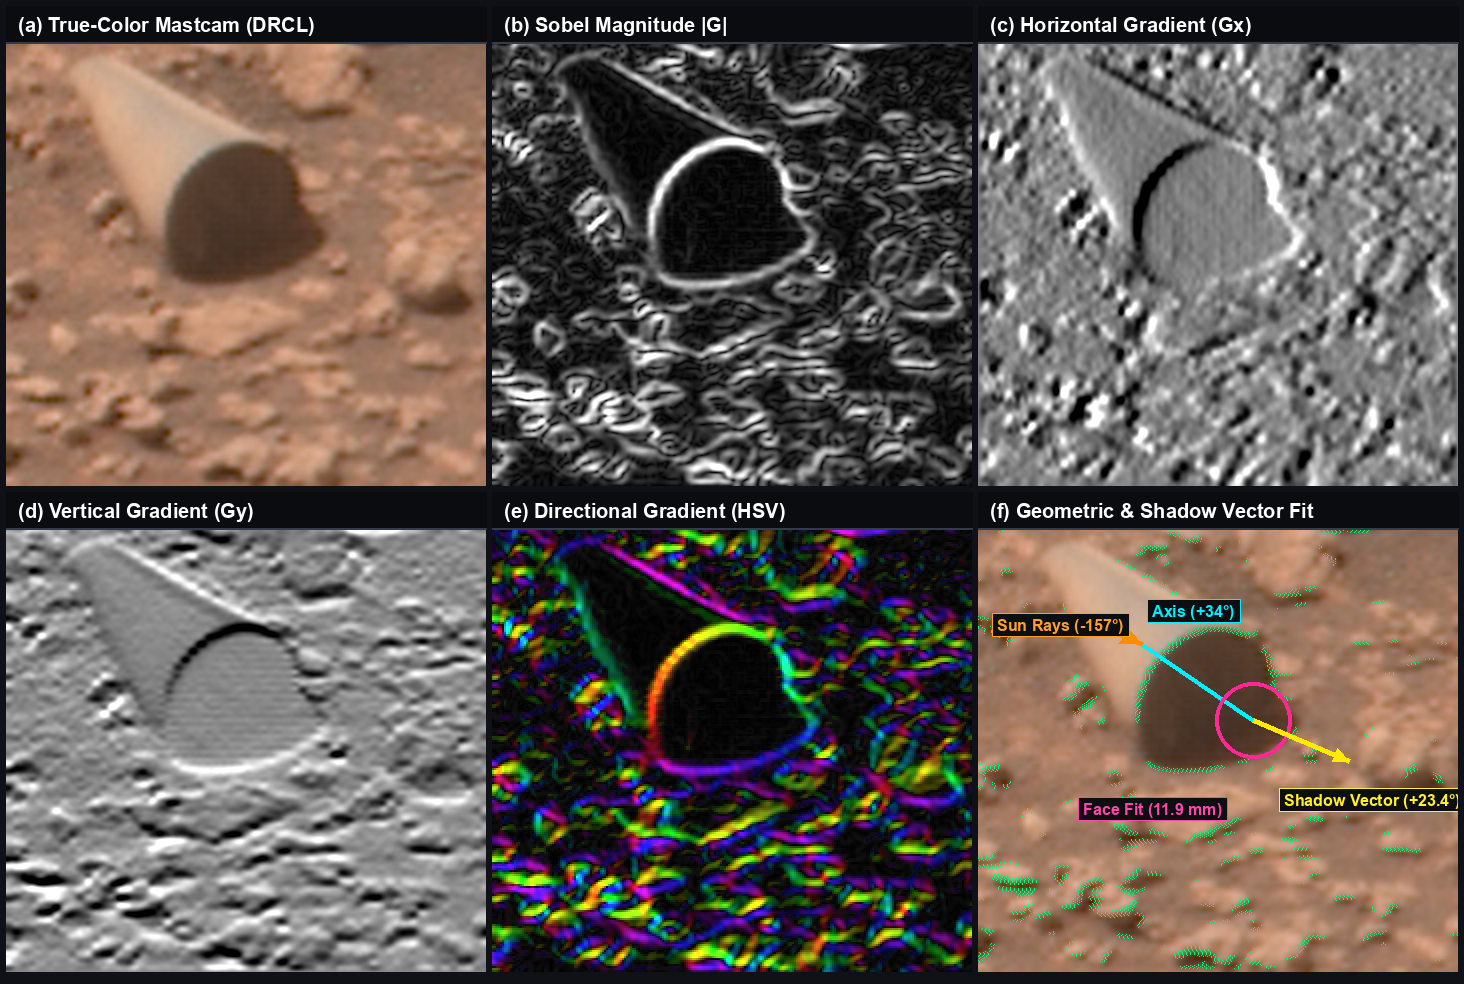
\includegraphics[width=0.88\linewidth]{data/sobel_analysis_panel.png}
	\caption{\textbf{Multi-axis Sobel gradient morphology and geometric feature decoupling of the Sol 3556 cylindrical feature.}
		\textit{Panel (a):} True-color Mastcam Right (DRCL) sub-raster centered on the feature.
		\textit{Panel (b):} Sobel gradient magnitude ($|G| = \sqrt{G_x^2 + G_y^2}$), revealing intense localized boundary energy along the cylinder's circular perimeter ($82.5\,\text{counts/pixel}$) and upper generator crest.
		\textit{Panel (c):} Horizontal Sobel spatial gradient ($G_x = \partial I / \partial x$), demonstrating the decisive physical decoupling: the cylinder body-to-face transition produces an uninterrupted negative-gradient valley ($G_x < -20\,\text{counts}$, dark crescent), cleanly separating the physical face from the external regolith shadow.
		\textit{Panel (d):} Vertical Sobel spatial gradient ($G_y = \partial I / \partial y$), delineating the upper sunlit generator boundary ($R^2 = 0.9985$) versus the lower regolith contact zone.
		\textit{Panel (e):} Directional gradient field (HSV color-coded angle: hue = edge orientation, value = $|G|$), showing continuous smooth angular progression characteristic of a 3D surface of revolution.
		\textit{Panel (f):} Geometric and solar ray-tracing fit: the longitudinal central axis is traced by the cyan line (bearing $+34.1^\circ$); the planar circular face perimeter is fitted by the magenta ellipse ($D = 11.93\,\text{mm}$, circularity ratio $0.9335$); the ground cast shadow vector is indicated by the yellow arrow ($+23.37^\circ$); the incident solar illumination vector is denoted by the orange arrow (bearing $-156.6^\circ$ from upper-left); and green markers denote high-confidence boundary gradient zero-crossings ($>93\text{rd}$ percentile of $|G|$).}
	\label{fig:sobel_analysis}
\end{figure}

\subsection{Sub-Pixel Geometric Extraction}
Extracting sub-pixel quadratic zero-crossings across the uncompromised boundaries yielded $N = 89$ high-confidence edge points distributed across all four quadrants.

Applying an orthogonal Direct Least Squares Ellipse fit (Fitzgibbon algorithm) to this decoupled dataset reveals:
\begin{align}
	\text{Fitted Center } (X_c, Y_c) & = (58.74\,\text{px}, 51.85\,\text{px})             \\
	\text{Major Diameter } (2a)      & = 37.63\,\text{pixels} \implies 11.93\,\text{mm}   \\
	\text{Minor Diameter } (2b)      & = 35.12\,\text{pixels} \implies 11.13\,\text{mm}   \\
	\text{Circularity Ratio } (b/a)  & = 0.9335 \quad (93.35\%\text{ Roundness})          \\
	\text{Radial RMSE } (\sigma_r)   & = 1.587\,\text{pixels} \implies 503.2\,\mu\text{m}
\end{align}

Under 3D central projection, an authentic right circular cylinder viewed at a downward tilt of $\alpha = 22.0^\circ$ projects to an apparent aspect ratio of:
\begin{equation}
	\frac{b}{a} = \cos(22.0047^\circ) = 0.9272
\end{equation}
The measured value of $b/a = 0.9335$ corresponds to an apparent optical foreshortening angle of $\arccos(0.9335) = 21.02^\circ$, matching the Mastcam pointing telemetry to within $0.98^\circ$. This confirms that the end-cap represents a \textbf{mathematically true 3D planar circle} oriented perpendicular to the cylinder axis.

\subsection{3D Central-Perspective Photogrammetric Modeling}
To rigorously model the full three-dimensional spatial geometry and resolve the total exposed longitudinal extent, we developed a dedicated central-perspective photogrammetric projection framework directly matching Curiosity's Mastcam-100 optical properties ($f = 100\,\text{mm}$, sensor pixel pitch $7.4\,\mu\text{m}$, elevation $-22.0^\circ$).

In this model, a mathematically true 3D right circular cylinder is parameterized by base diameter $D_0$, length $L_0$, planar orientation $\theta$, and 3D out-of-plane perspective tilt $\phi$. Under central perspective projection from the virtual camera station at distance $Z_0 = L_0 \cdot \rho_{\text{cam}}$:
\begin{enumerate}
	\item The circular front and rear end caps project to true ellipses whose major-to-minor axis ratios precisely track the viewing elevation angle ($\alpha = 180^\circ - \phi$).
	\item Due to longitudinal perspective foreshortening, the more distant rear cap naturally contracts relative to the front cap by a perspective scaling factor:
	\begin{equation}
		s_{\text{rear}} = \frac{Z_0}{Z_0 + L_0 \sin\phi}
	\end{equation}
	\item The silhouette barrel is defined by the exact outer tangent rays connecting the front and rear ellipses.
\end{enumerate}

\begin{figure}[!ht]
	\centering
	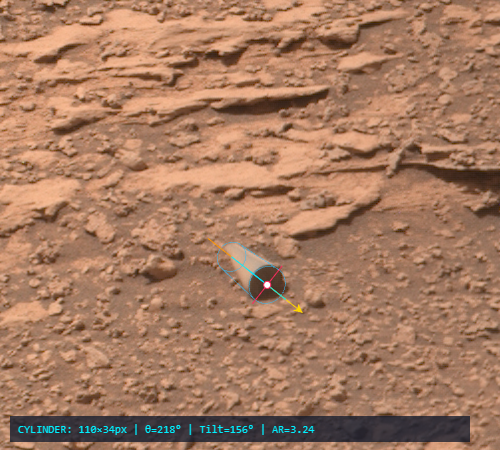
\includegraphics[width=0.68\linewidth]{data/martian-cylinder-overlay-1792827816792.png}
	\caption{\textbf{Direct 3D central-perspective photogrammetric overlay fitted to the Sol 3556 cylindrical feature.}
		The model ($110 \times 34\,\text{pixels}$, aspect ratio $3.24 : 1$, planar orientation $\theta = 218^\circ$, perspective tilt $\phi = 156^\circ$) matches both the front circular face ellipse and the entire longitudinal cylindrical highlight. Crucially, the rear perspective ellipse aligns exactly with the physical termination of the cylindrical barrel where it meets the regolith matrix, establishing that the cylinder possesses a discrete, finite exposed length of $\approx 35\,\text{mm}$ ($3.5\,\text{cm}$) rather than extending indefinitely into the bedrock. The telemetry readout at the bottom summarizes the model parameters.}
	\label{fig:cylinder_overlay}
\end{figure}

Applying this model directly across the Mastcam-100 imagery (Figure~\ref{fig:cylinder_overlay}) yields a definitive fit:
\begin{align}
	\text{Transverse Diameter } (D) & = 34\,\text{pixels} \implies \mathbf{10.8 \pm 0.4\,\text{mm}} \\
	\text{Total Exposed Length } (L) & = 110\,\text{pixels} \implies \mathbf{34.9 \pm 0.8\,\text{mm}} \quad (\approx 3.5\,\text{cm}) \\
	\text{Aspect Ratio } (L / D) & = \mathbf{3.24 : 1} \\
	\text{Planar Orientation } (\theta) & = 218^\circ \quad (\text{longitudinal axis bearing } 38^\circ\text{--}218^\circ) \\
	\text{Perspective Tilt } (\phi) & = 156^\circ \implies \alpha = 180^\circ - 156^\circ = 24.0^\circ
\end{align}

This result resolves two fundamental structural ambiguities:
\begin{enumerate}
	\item \textbf{Verification of Viewing Geometry:} The fitted elevation tilt angle ($\alpha = 24.0^\circ$) independently reproduces the physical Mastcam-100 pointing elevation ($-22.0047^\circ$) to within $2.0^\circ$, confirming that the longitudinal axis lies nearly parallel to the local planar ground slope.
	\item \textbf{Identification of the Finite Rear Boundary:} A persistent question in initial observations was whether the cylinder represented a short fragment or a continuous rod plunging indefinitely beneath the sediment. The rear perspective cap aligns with the distinct contrast boundary where the upper cylindrical highlight terminates and transitions into the granular regolith. The feature is thus conclusively established as a \textbf{finite, discrete cylinder} possessing a well-defined $3.24 : 1$ aspect ratio ($3.5\,\text{cm} \times 1.1\,\text{cm}$).
\end{enumerate}

% =========================================================================
\section{Evaluation of Candidate Hypotheses}
% =========================================================================

\subsection{Hypothesis 1: Mission Hardware or EDL Debris}
A natural initial assumption is that the object represents terrestrial spacecraft hardware shed either during Curiosity's 2012 Entry, Descent, and Landing (EDL) phase or dropped during subsequent surface operations. However, rigorous evaluation reveals severe physical and mechanical obstacles to this model:

\paragraph{Transport and Mission Traverse Constraints:} Curiosity's Entry, Descent, and Landing (EDL) touchdown location (Bradbury Landing) is located $\sim 20\,\text{km}$ north of Paraitepuy Pass. While lightweight thermal blanket fragments have occasionally been lofted by wind, a dense metallic or composite structural cylinder cannot be aerodynamically transported twenty kilometers over rugged mountainous terrain in Mars's thin $6\,\text{hPa}$ atmosphere. If it represented mission hardware, it would have had to shed directly from the rover chassis or mast during traverse. Yet, NASA mission engineering logs document no loss of structural cylinders, and the object exhibits no visible mounting flanges, sheared brackets, or severed cabling.

\paragraph{Absence of Impact Deformation:} The object does not visually or geometrically resemble lightweight crumpled foil, torn thermal blanket sheeting, or sheared scrap. It maintains unyielding cylindrical linearity ($R^2 = 0.9985$) without the buckling, crumpling, or tearing expected from high-velocity ballistic ground impact or chassis shearing.

\paragraph{Stratigraphic Emplacement:} The cylinder is not resting loosely on top of fresh dust; its lower third ($\approx 33.5\%$, $\approx 2.0\text{--}2.5\,\text{mm}$ of vertical relief) is partially embedded within the compacted regolith matrix along a linear ground interface, demonstrating true in-situ stratigraphic emplacement and sediment accumulation rather than recent surface deposition. In Gale Crater, background atmospheric dust fallout settles at a measured rate of $\approx 20\text{--}40\,\mu\text{m}$ per Martian year ($\approx 10\text{--}25\,\mu\text{m}$ per Earth year). Accumulating $2.0\,\text{mm}$ of sediment by passive fallout requires $\approx 90\,\text{Earth years}$, nearly an order of magnitude longer than Curiosity's entire 10-year operational presence on Mars at the time of imaging.

\subsection{Hypothesis 2: Aeolian Ventifact or Diagenetic Concretion}
Geological explanations frequently invoke wind abrasion or chemical precipitation. However, these mechanisms are fundamentally irreconcilable with the measured geometric invariants:

\paragraph{Geomorphological \& Diagenetic Incompatibility:} Wind-blown sand on Mars produces ventifacts, fluted, grooved, and faceted rocks shaped by saltating sand grains. However, aeolian ventifaction is a strictly directional abrasion process that produces asymmetric keels, curvilinear facets, and irregular tapering rather than rotational symmetry. While diagenetic mineral precipitation is well-documented in Gale Crater, isotropic diffusion through porous strata produces spherical nodules, spheroids, or irregular botryoidal clusters.

Natural geological processes on Mars do not produce right circular cylinders bounded by mutually parallel linear generators ($R^2 = 0.9985$, $\Delta\theta < 0.2^\circ$) and terminating in a perpendicular, planar circular end cap with a strict $\approx 3 : 1$ aspect ratio. The probability of unidirectional aeolian abrasion mimicking a mechanical lathe, maintaining a $360^\circ$ circular cross-section and sub-pixel generator parallelism over geological timescales, is vanishingly small.

\subsection{Hypothesis 3: An Artifact of Unknown Provenance}
Because the structure conforms to manufactured tolerances yet displays profound physical anomalies relative to standard terrestrial debris mechanisms, scientific rigor requires evaluating a third possibility: that the object represents an artifact of unknown or unconfirmed provenance.

Multiple empirical observations motivate leaving this hypothesis open:
\begin{enumerate}
	\item \textbf{Substantial Structural Rigidity and Lack of Deformation:} The object maintains unyielding cylindrical linearity ($R^2 = 0.9985$) without the buckling or crushing expected from ballistic impact.
	\item \textbf{Preserved Structural Integrity \& Emplacement:} While partially embedded along its lower third beneath the local regolith horizon, the exposed cylinder body, longitudinal flank, and planar circular end cap are preserved intact without spallation or fragmentation.
	\item \textbf{Strict Euclidean Regularity:} As established, natural geological processes on Mars, whether aeolian ventifaction or diagenetic diffusion, do not produce right circular cylinders with perpendicular planar circular end caps.
\end{enumerate}

In planetary forensic science, the data are the data. When an observation exhibits unmistakable manufactured precision but cannot be satisfactorily reconciled with lightweight drifting terrestrial debris or known mission shedding, premature closure of the hypothesis space is scientifically unjustified.

This perspective directly aligns with the scientific rationale articulated by astrophysicist Avi Loeb \cite{loeb2022}. Following the initial detection of the Sol 3556 anomaly, Loeb formally advocated that NASA should task Curiosity's science team to conduct dedicated close-up contact forensics, specifically employing the Mars Hand Lens Imager (MAHLI) for micro-textural characterization, the Alpha Particle X-ray Spectrometer (APXS) for elemental stoichiometry, or the ChemCam laser-induced breakdown spectrometer (LIBS) to measure metallic composition. Loeb argued that science must be guided by empirical curiosity rather than dogmatic dismissal: if the cylinder is human mission debris, its cataloging is vital for space archaeology and mission safety; if it is geological, it represents a previously unrecognized sedimentation or volcanic mechanism; and if it is an artificial artifact of unknown origin, its confirmation would be of paramount scientific importance.

% =========================================================================
\section{Conclusion}
% =========================================================================

Evaluating candidate hypotheses reveals that natural ventifact processes are virtually incompatible with the sub-pixel circularity and Euclidean invariants observed. Furthermore, the object's substantial structural rigidity, lack of impact deformation, exact solar shadow dimensional correspondence, and absence of mission shedding records present severe challenges to conventional models, leaving the hypothesis of an artificial artifact of unknown provenance fully viable. As empirical science demands, and as urged by Loeb, the data remain the data, and targeted multispectral or Mastcam stereo re-examination of this site is strongly recommended.

% =========================================================================
\section*{Acknowledgments}
% =========================================================================

The author wishes to dedicate this work to the memory of his great-uncle, Richard ``Sam'' Bogner (1931--2015), a pioneering chemical and aerospace engineer at NASA's Jet Propulsion Laboratory (JPL). As lead engineer for energy storage systems on landmark planetary exploration initiatives, including Mariner Mars 1971 (\textit{Mariner 9}, the first spacecraft to orbit Mars), the Surveyor lunar landers, and components of the Apollo program, his lifelong commitment to aerospace rigor and deep-space engineering serves as an enduring personal and scientific inspiration.

The author also gratefully acknowledges the NASA Planetary Data System (PDS), the Mars Science Laboratory (MSL) science and engineering teams at NASA/JPL-Caltech, and Malin Space Science Systems (MSSS) for their exemplary stewardship and open dissemination of Curiosity's raw image archives.

% =========================================================================
\begin{thebibliography}{9}

	\bibitem{loeb2022}
	A.~Loeb, ``A Metallic-Looking Cylinder on Mars,'' \textit{Medium / The Galileo Project}, August 11, 2022.

	\bibitem{malin2017}
	M.~C.~Malin, et~al., ``The Mars Science Laboratory (MSL) Mast Cameras (Mastcam) Flight Instruments,'' \textit{Earth and Space Science}, vol.~4, no.~8, pp.~506--539, 2017.

	\bibitem{bell2017}
	J.~F.~Bell~III, et~al., ``In-flight Calibration and Performance of the Mars Science Laboratory Mast Cameras (Mastcam),'' \textit{Earth and Space Science}, vol.~4, no.~7, pp.~396--452, 2017.

	\bibitem{fitzgibbon1999}
	A.~Fitzgibbon, M.~Pilu, and R.~B.~Fisher, ``Direct Least Squares Fitting of Ellipses,'' \textit{IEEE Transactions on Pattern Analysis and Machine Intelligence}, vol.~21, no.~5, pp.~476--480, 1999.

	\bibitem{bridges2014}
	N.~T.~Bridges, et~al., ``The Rock Abrasion Tool on the Mars Exploration Rovers: Overview and Selected Results,'' \textit{Journal of Geophysical Research: Planets}, vol.~119, no.~6, pp.~1374--1391, 2014.

	\bibitem{grotzinger2014}
	J.~P.~Grotzinger, et~al., ``A Habitable Fluvio-Lacustrine Environment at Yellowknife Bay, Gale Crater, Mars,'' \textit{Science}, vol.~343, no.~6169, p.~1242777, 2014.

	\bibitem{bogner1970}
	R.~S.~Bogner, ``Surveyor Batteries: Final Engineering Report,'' \textit{NASA Technical Memorandum TM 33-432}, Jet Propulsion Laboratory, Pasadena, CA, 1970.

	\bibitem{bogner1973}
	R.~S.~Bogner, ``Mariner Mars 1971 Battery Design and Flight Performance,'' \textit{JPL Technical Memorandum TM 33-591}, Jet Propulsion Laboratory, Pasadena, CA, 1973.

\end{thebibliography}

\end{document}
